\chapter{Results}\label{chap:results}

\section{Experiment 1: German Credit}

\subsection{Prediction Invariance}

The test \gls{RMSE} is 2043.3 across all three weighting modes ($\wemp$, $\wunif$, $\windep$), confirming that purification does not alter predictions.
The maximum absolute prediction error between the original XGBoost model and the purified tensor representation is below $10^{-2}$ in all cases.

\subsection{Dominant Effects}

\Cref{tab:german-mains,tab:german-interactions} show the top main effects and interactions ranked by variance under $\wemp$.
\texttt{Duration} dominates (variance $\approx 2.9 \times 10^6$); the strongest interaction is \texttt{Duration} $\times$ \texttt{Purpose\_vacation} ($\approx 29{,}522$).

\begin{table}[H]
\centering
\small
\caption[Top main effects in the German Credit experiment.]{Top main effects ranked by weighted variance under $\wemp$.}
\begin{tabular}{lr}
\toprule
\textbf{Feature} & \textbf{Variance} \\
\midrule
Duration & 2,906,619 \\
Job\_3 & 247,365 \\
Purpose\_vacation & 93,542 \\
Age & 79,656 \\
Purpose\_radio/TV & 43,529 \\
Purpose\_education & 9,319 \\
\bottomrule
\end{tabular}
\label{tab:german-mains}
\end{table}

\begin{table}[H]
\centering
\small
\caption[Top interactions in the German Credit experiment.]{Top pairwise interactions ranked by weighted variance under $\wemp$.}
\begin{tabular}{lr}
\toprule
\textbf{Feature pair} & \textbf{Variance} \\
\midrule
Duration $\times$ Purpose\_vacation & 29,522 \\
Age $\times$ Duration & 17,139 \\
Duration $\times$ Job\_3 & 7,498 \\
Saving\_moderate $\times$ Purpose\_education & 5,888 \\
Sex\_female $\times$ Purpose\_education & 3,015 \\
\bottomrule
\end{tabular}
\label{tab:german-interactions}
\end{table}

\subsection{Main Effect Sensitivity to Weights}

\Cref{fig:german-mains} shows the purified main effect curves under the three weight modes.
The overall shape is preserved, but magnitudes and vertical offsets differ, reflecting variance reallocation between mains and interactions.

\begin{figure}[H]
\centering
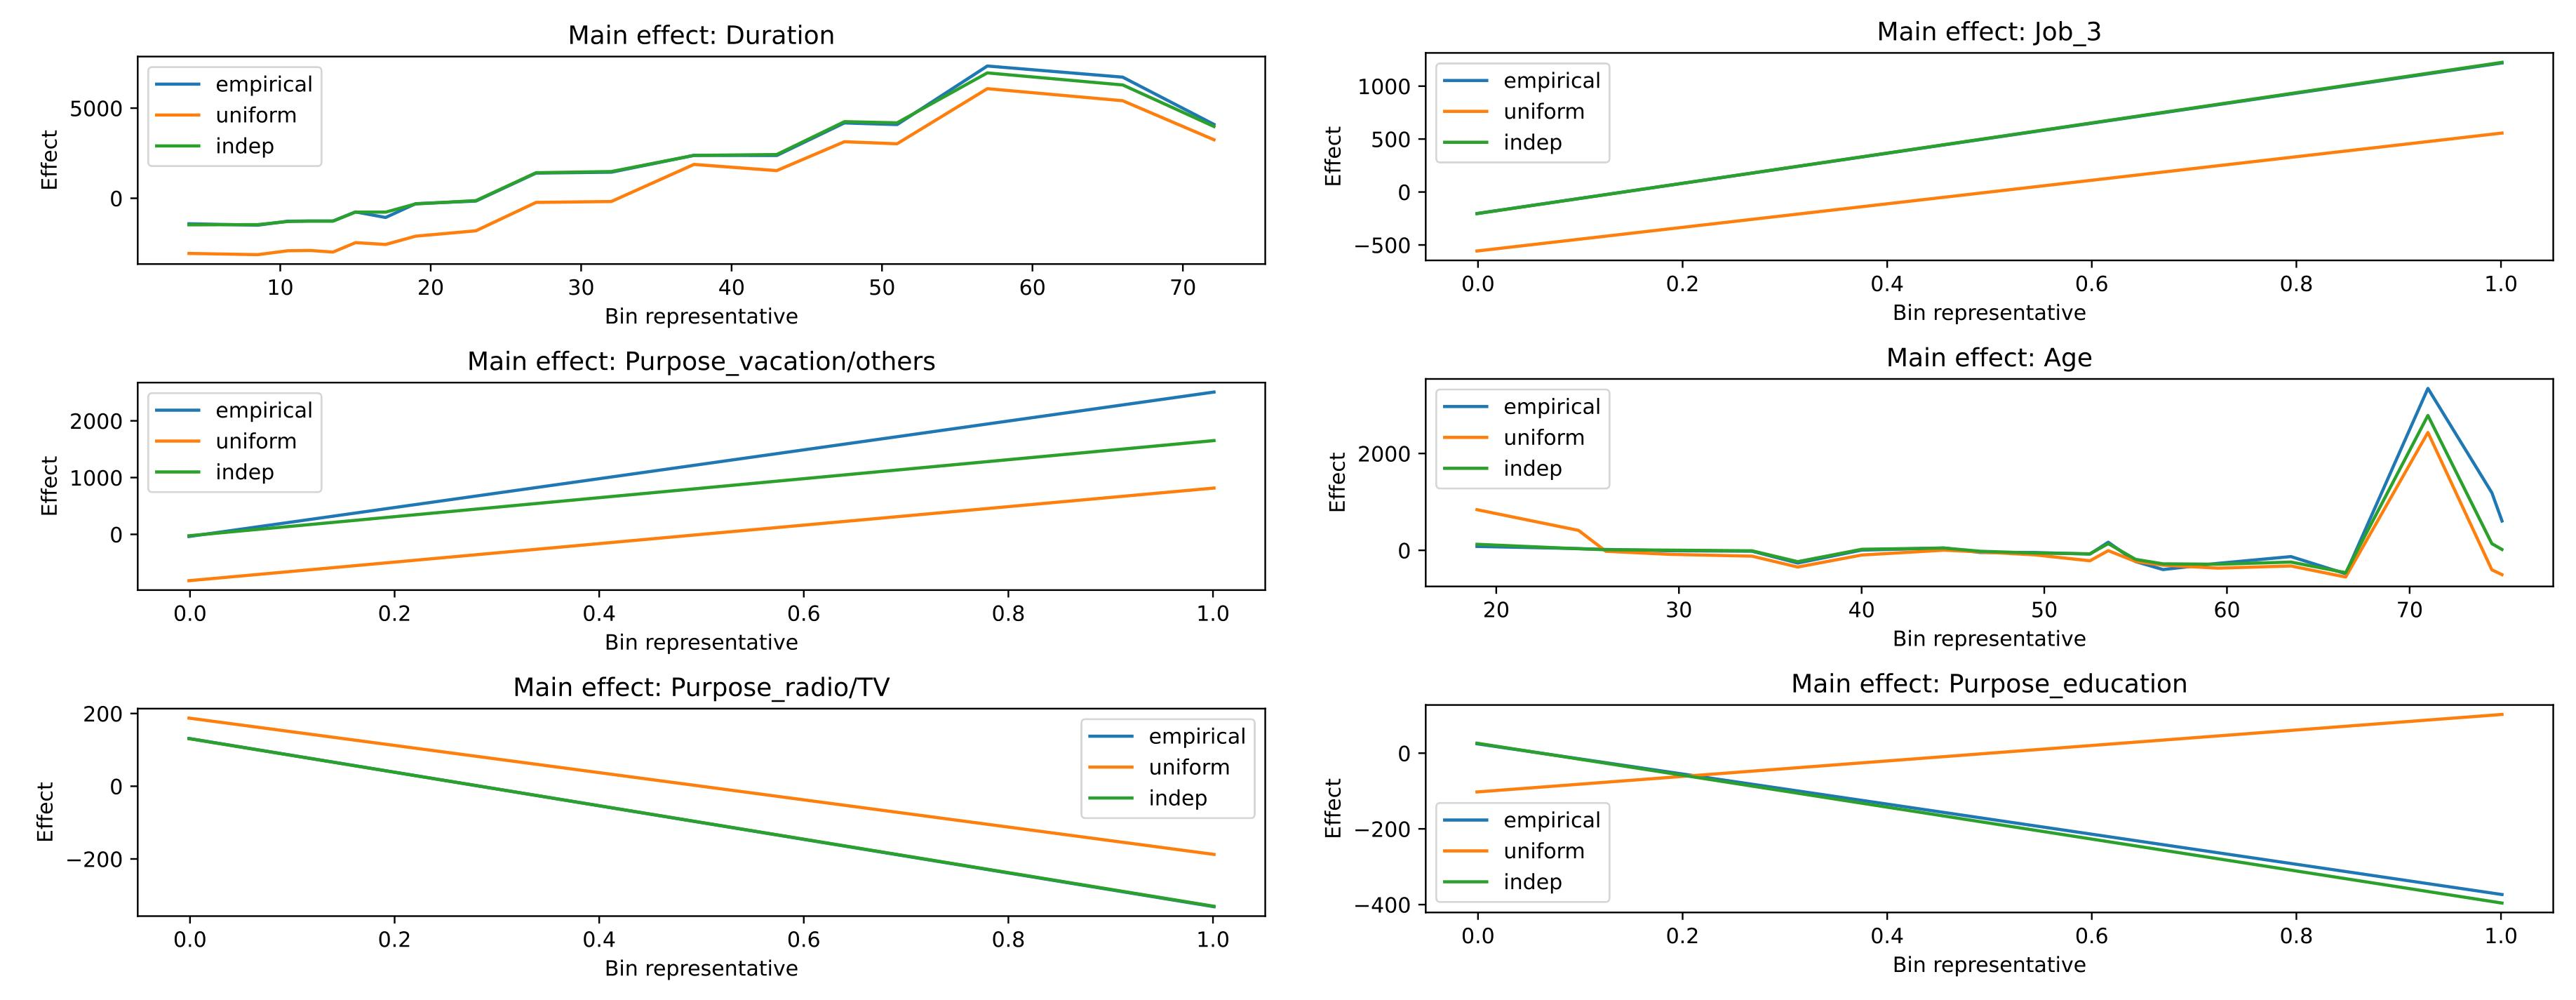
\includegraphics[width=\textwidth,height=0.45\textheight,keepaspectratio]{german_credit_top_mains.pdf}
\caption[German Credit: main effect curves under different weight modes.]{Purified main effect curves for the top features under $\wemp$ (blue), $\wunif$ (orange), and $\windep$ (green). Predictions are identical across all modes.}
\label{fig:german-mains}
\end{figure}

\subsection{Interaction Heatmaps}

\Cref{fig:german-heatmap} shows the top interaction surface before and after purification under each weight mode.
The unpurified interaction contains substantial marginal structure; after purification, the qualitative pattern of the residual differs across weight modes.

\begin{figure}[H]
\centering
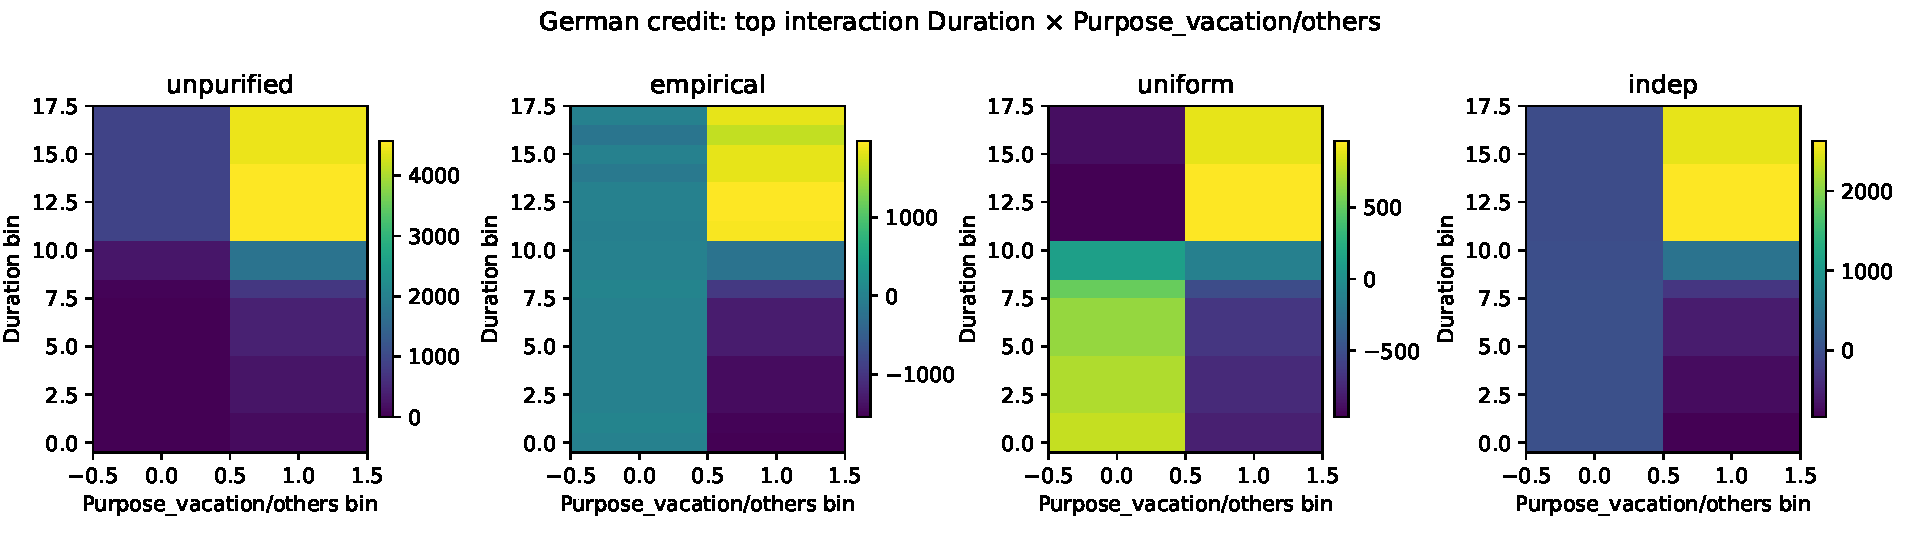
\includegraphics[width=0.85\textwidth,height=0.4\textheight,keepaspectratio]{german_credit_top_interaction_heatmap.pdf}
\caption[German Credit: interaction heatmaps.]{Top interaction surface (Duration $\times$ Purpose\_vacation) before purification (leftmost) and after purification under $\wemp$, $\wunif$, and $\windep$.}
\label{fig:german-heatmap}
\end{figure}

\section{Experiment 2: Stress-Test Under Controlled Dependence}

All metrics are reported relative to the $\wemp$-purified baseline.
For each metric, we show F1 (multiplicative, expected to be more robust) and F2 (XOR-like, expected to be more sensitive).

\subsection{$L_2$ Distance vs.\ Dependence Strength}

For F1 (\cref{fig:stress-l2-F1}), the $L_2$ distance remains moderate (0.27--0.32 at $\rhoVal = 0.97$).
For F2 (\cref{fig:stress-l2-F2}), the picture changes dramatically: at $\rhoVal = 0.97$, the $L_2$ distance reaches 0.87--0.90---the purified surface is nearly unrecognizable compared to the $\wemp$ baseline.

\begin{figure}[H]
\centering
\subfloat[F1 (multiplicative)\label{fig:stress-l2-F1}]{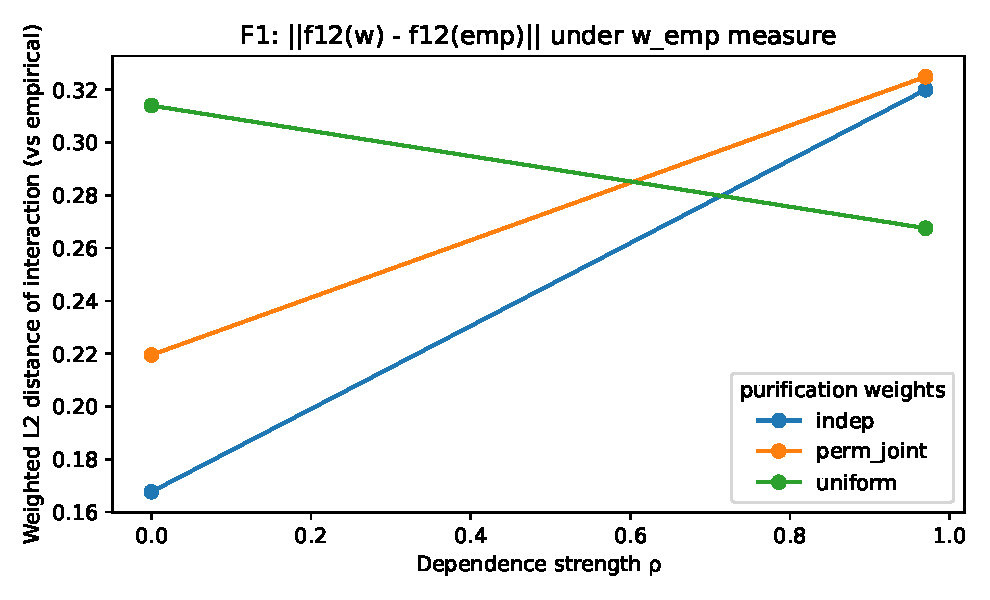
\includegraphics[width=0.48\textwidth]{stress_dependence_l2_interaction_F1.pdf}}%
\hfill%
\subfloat[F2 (XOR-like)\label{fig:stress-l2-F2}]{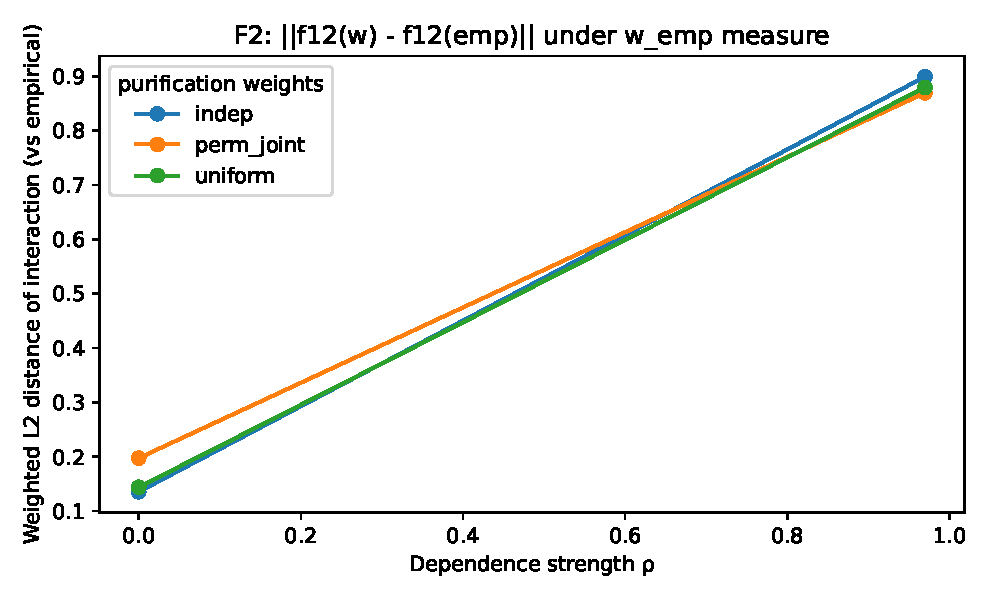
\includegraphics[width=0.48\textwidth]{stress_dependence_l2_interaction_F2.pdf}}
\caption[Stress-test: $L_2$ distance vs.\ $\rhoVal$.]{Weighted $L_2$ distance from the $\wemp$ baseline. F1 (left) remains moderate; F2 (right) approaches 0.9 at high $\rhoVal$.}
\label{fig:stress-l2}
\end{figure}

\subsection{Sign Flip Rate}

For F1 (\cref{fig:stress-signflip-F1}), sign flips are negligible at low $\rhoVal$ but reach 29--34\% at $\rhoVal = 0.97$---roughly a third of bins reverse their interpretation.
For F2 (\cref{fig:stress-signflip-F2}), the rate is lower (17--19\%) despite F2's larger $L_2$ distance, because the XOR-like interaction has large absolute values in all quadrants---sign flips occur mainly near the zero-crossing boundaries.

\begin{figure}[H]
\centering
\subfloat[F1 (multiplicative)\label{fig:stress-signflip-F1}]{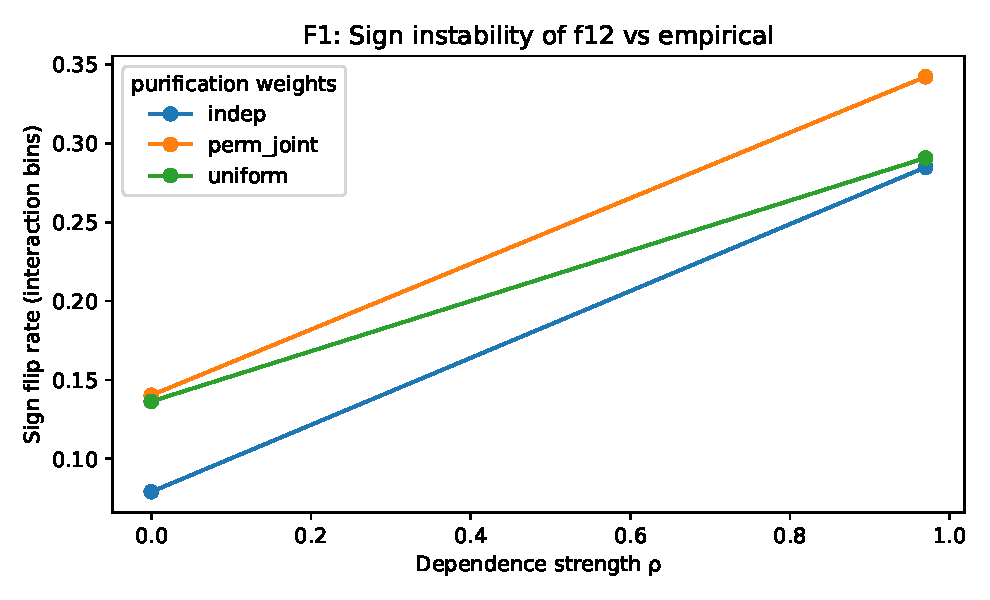
\includegraphics[width=0.48\textwidth]{stress_dependence_signflip_interaction_F1.pdf}}%
\hfill%
\subfloat[F2 (XOR-like)\label{fig:stress-signflip-F2}]{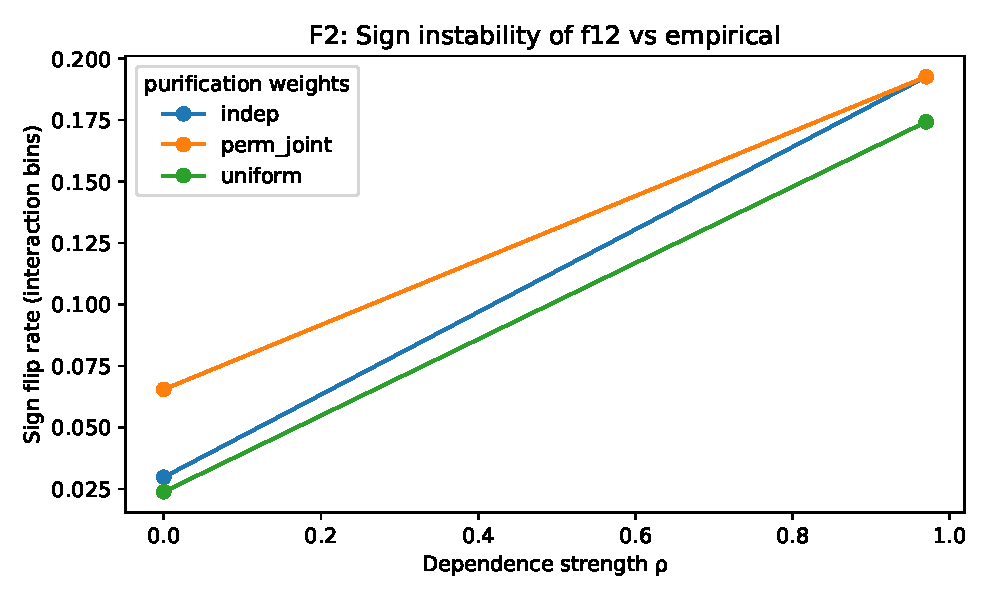
\includegraphics[width=0.48\textwidth]{stress_dependence_signflip_interaction_F2.pdf}}
\caption[Stress-test: sign flip rate vs.\ $\rhoVal$.]{Fraction of interaction bins whose sign differs from the $\wemp$ baseline. F1 (left) reaches 29--34\%; F2 (right) reaches 17--19\% at high $\rhoVal$.}
\label{fig:stress-signflip}
\end{figure}

\subsection{Interaction Variance Share}

The interaction variance share determines the high-level narrative: ``Is this model dominated by main effects, or does the interaction matter?''
For F1 (\cref{fig:stress-share-F1}), the share under $\wemp$ drops from 29\% at $\rhoVal = 0$ to essentially 0\% at $\rhoVal = 0.97$, while $\wunif$ and $\windep$ retain 1--6\%.
For F2 (\cref{fig:stress-share-F2}), the divergence is dramatic: at $\rhoVal = 0.97$, $\wemp$ reports 5.6\% while $\windep$ reports \textbf{73\%}---the same model and data yield diametrically opposed narratives depending solely on the weight specification.

\begin{figure}[H]
\centering
\subfloat[F1 (multiplicative)\label{fig:stress-share-F1}]{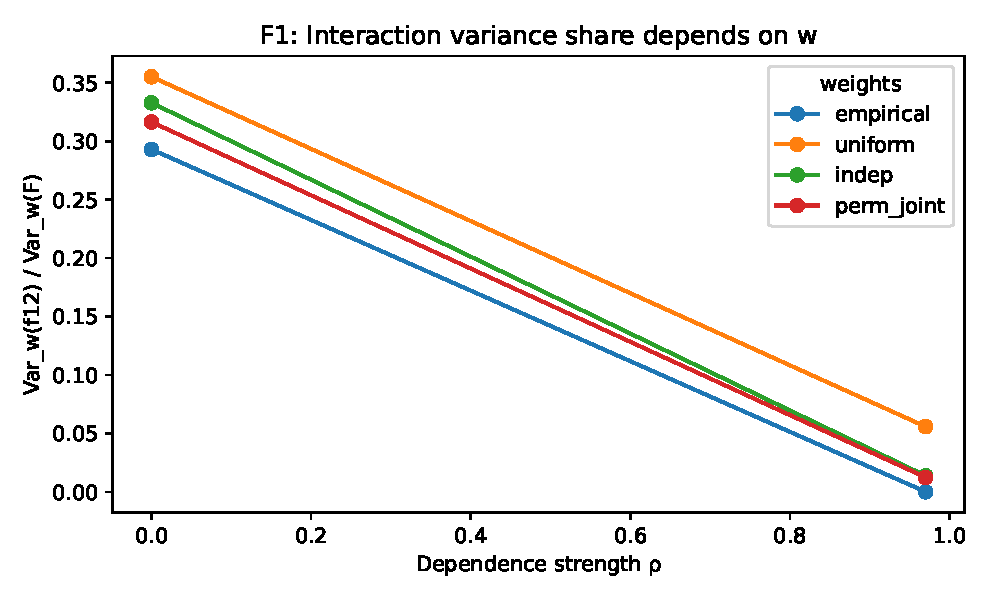
\includegraphics[width=0.48\textwidth]{stress_dependence_interaction_share_F1.pdf}}%
\hfill%
\subfloat[F2 (XOR-like)\label{fig:stress-share-F2}]{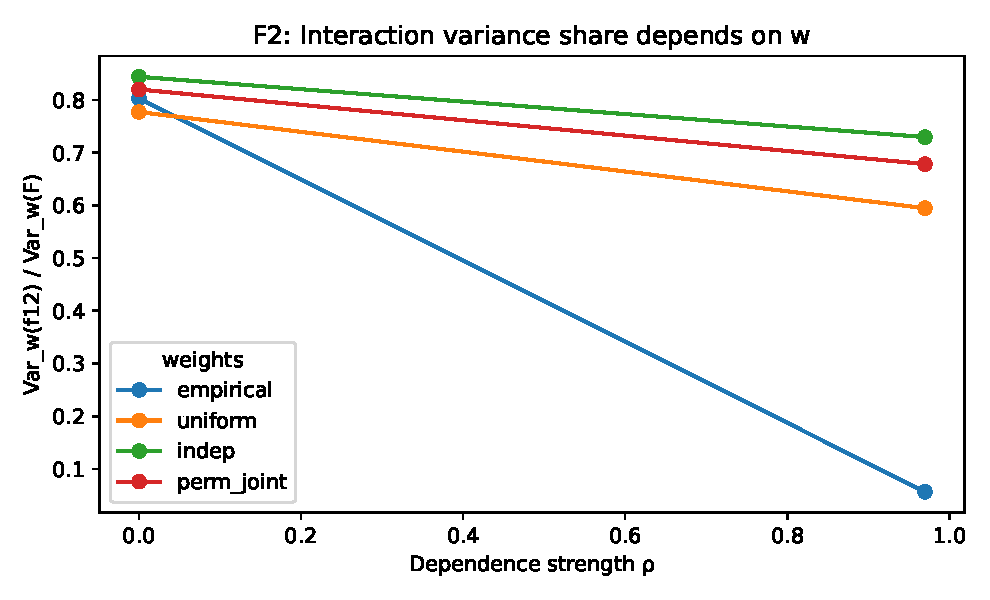
\includegraphics[width=0.48\textwidth]{stress_dependence_interaction_share_F2.pdf}}
\caption[Stress-test: interaction variance share vs.\ $\rhoVal$.]{Interaction variance share. F1 (left): $\wemp$ drops to $\approx$0\% at high $\rhoVal$. F2 (right): $\wemp$ reports 5.6\% while $\windep$ reports 73\%.}
\label{fig:stress-share}
\end{figure}

\subsection{Main Effects at Strong Dependence}

Where does the ``missing'' interaction variance go?
\Cref{fig:stress-mains-F1} shows the main effect curves for F1 at $\rhoVal = 0.97$: under $\wemp$, the mains are steeper (absorbing nearly all variance), while under $\windep$ and $\wunif$ they are flatter.

\begin{figure}[H]
\centering
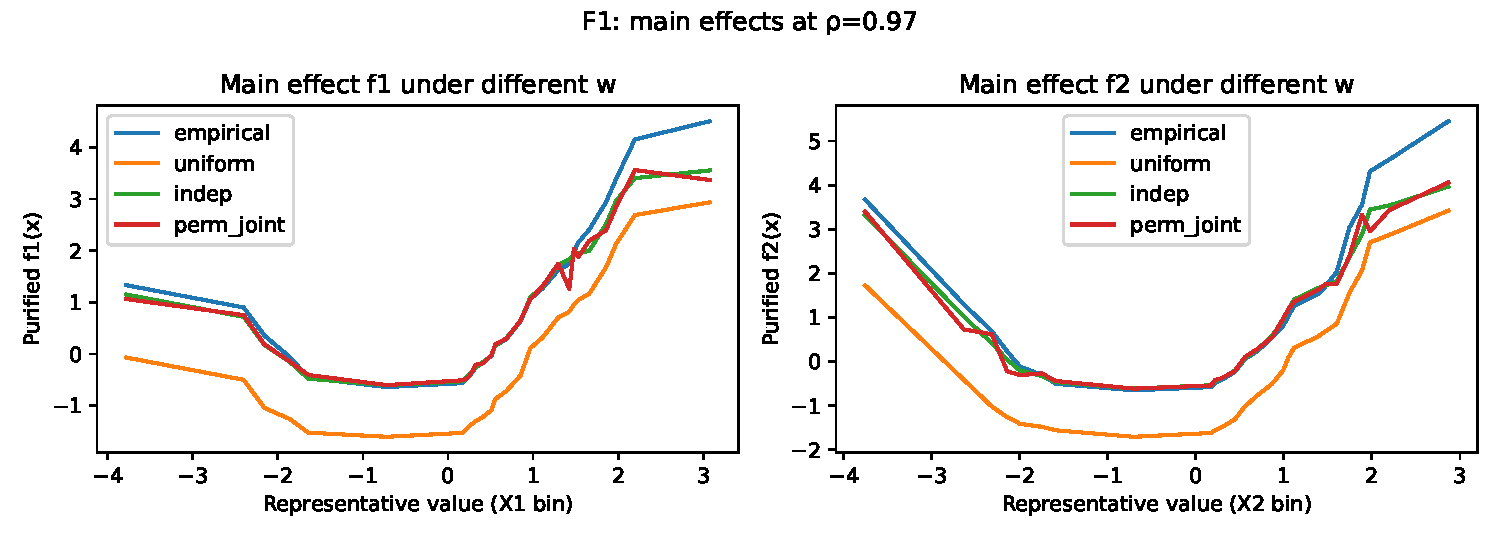
\includegraphics[width=0.75\textwidth,height=0.35\textheight,keepaspectratio]{stress_dependence_mains_F1_rho0.97.pdf}
\caption[Stress-test F1: main effect curves at $\rhoVal = 0.97$.]{F1 main effect curves at $\rhoVal = 0.97$. $\wemp$ curves are steeper; $\windep$ and $\wunif$ retain more interaction structure.}
\label{fig:stress-mains-F1}
\end{figure}

\subsection{Interaction Heatmaps at Strong Dependence}

\Cref{fig:stress-heatmaps-F1} shows the F1 interaction surface at $\rhoVal = 0.97$: under $\wemp$ the residual is nearly flat, while $\windep$ and $\wunif$ partially preserve the saddle structure.

\begin{figure}[H]
\centering
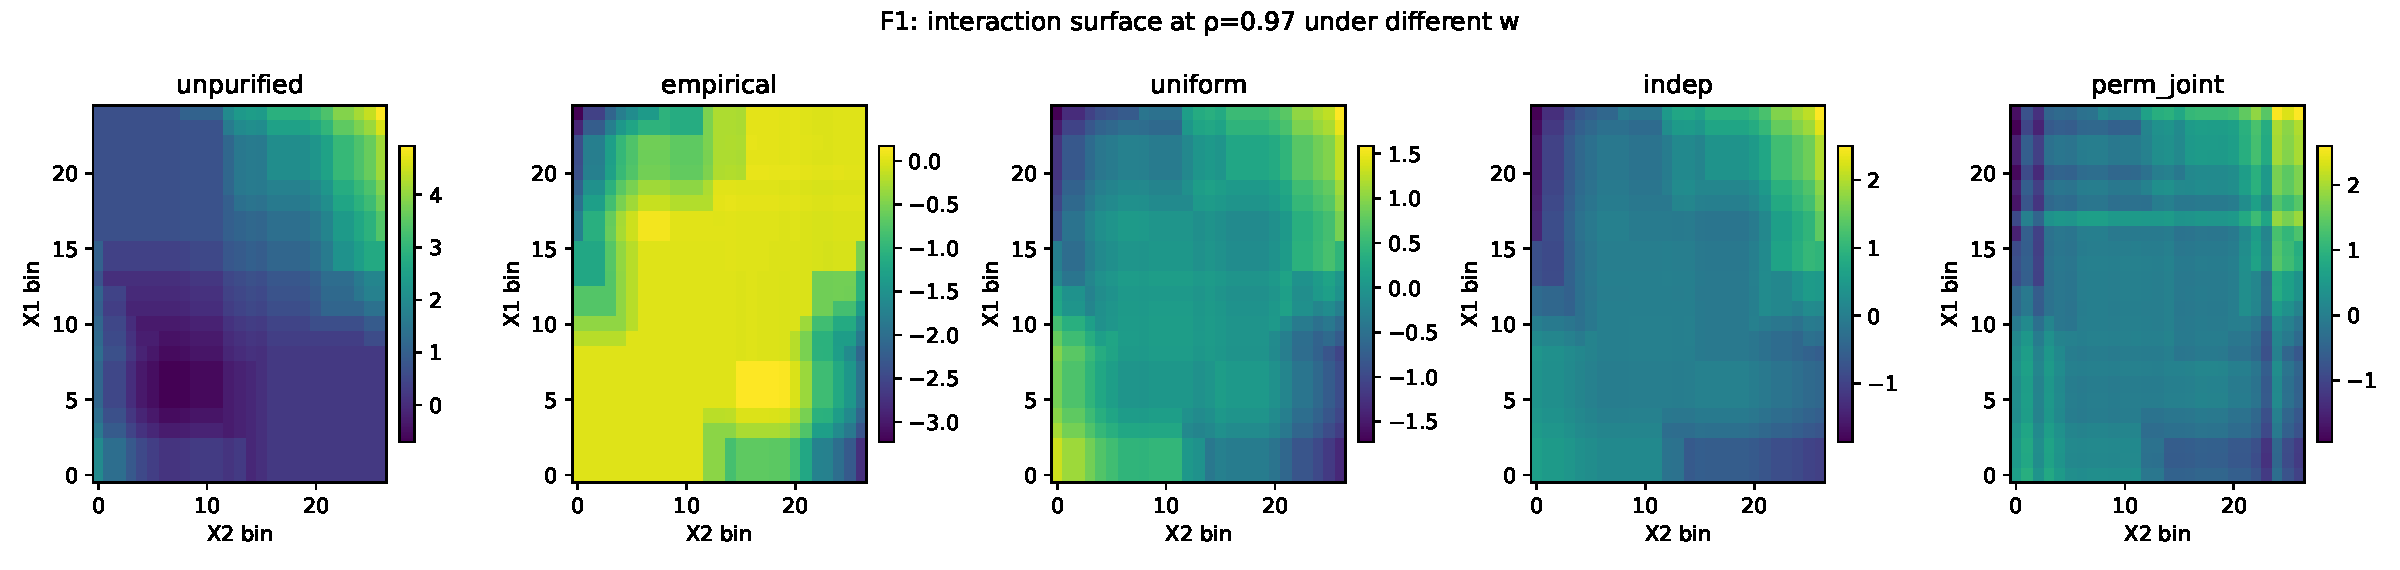
\includegraphics[width=0.8\textwidth,height=0.35\textheight,keepaspectratio]{stress_dependence_heatmaps_F1_rho0.97.pdf}
\caption[Stress-test F1: interaction heatmaps at $\rhoVal = 0.97$.]{F1 interaction surfaces at $\rhoVal = 0.97$: unpurified (leftmost), then purified under each weight mode.}
\label{fig:stress-heatmaps-F1}
\end{figure}

\Cref{fig:stress-heatmaps-F2} shows F2, where the contrast is most striking: the checkerboard pattern is clearly visible under $\windep$ and $\wunif$ but largely absent under $\wemp$.

\begin{figure}[H]
\centering
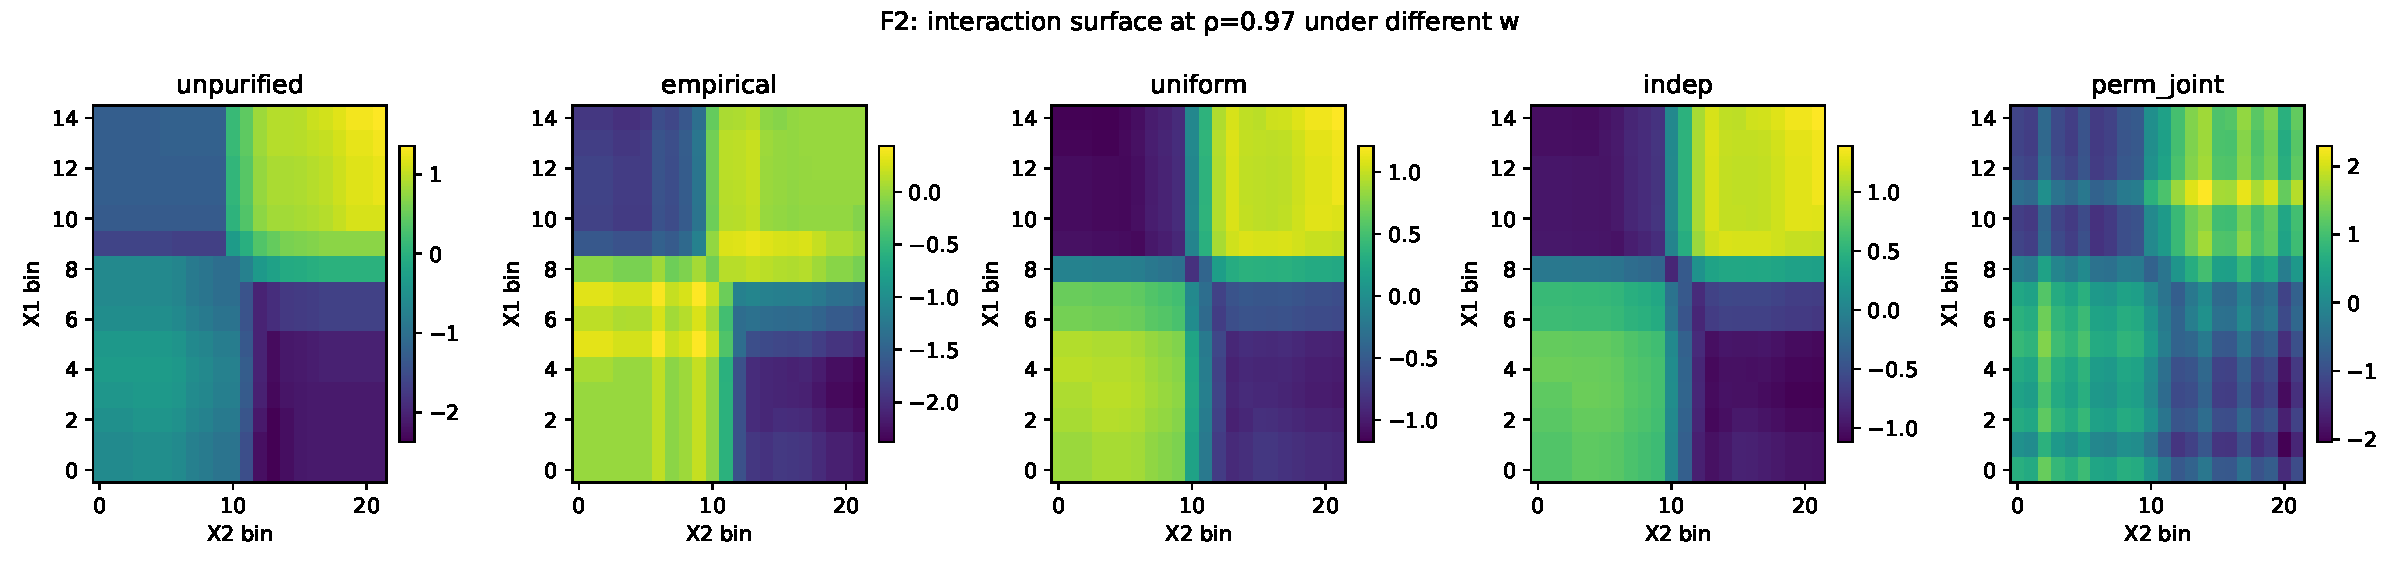
\includegraphics[width=0.8\textwidth,height=0.35\textheight,keepaspectratio]{stress_dependence_heatmaps_F2_rho0.97.pdf}
\caption[Stress-test F2: interaction heatmaps at $\rhoVal = 0.97$.]{F2 interaction surfaces at $\rhoVal = 0.97$. $\windep$ shows a strong checkerboard; $\wemp$ shows a much weaker pattern.}
\label{fig:stress-heatmaps-F2}
\end{figure}

\subsection{Summary of Stress-Test Results}

\Cref{tab:stress-summary} summarizes the key metrics at the extremes of dependence.
At $\rhoVal = 0$, all weight modes agree; at $\rhoVal = 0.97$, they diverge substantially.
F2 is more sensitive than F1 on every metric except sign flip rate, where F1's smoother surface leads to more sign reversals near zero crossings.

\begin{table}[H]
\centering
\small
\caption[Summary of stress-test results.]{Summary of stress-test metrics at $\rhoVal = 0$ and $\rhoVal = 0.97$ for both ground-truth functions. Interaction variance share is given for each weight mode; $L_2$ distance and sign flip rate are reported for non-empirical modes against the $\wemp$ baseline.}
\begin{tabular}{l|cc|cc}
\toprule
 & \multicolumn{2}{c|}{\textbf{F1 (multiplicative)}} & \multicolumn{2}{c}{\textbf{F2 (XOR-like)}} \\
\textbf{Metric / Mode} & $\rhoVal{=}0$ & $\rhoVal{=}0.97$ & $\rhoVal{=}0$ & $\rhoVal{=}0.97$ \\
\midrule
\multicolumn{5}{l}{\textit{Interaction variance share (\%)}} \\
\quad $\wemp$ & 29 & $\approx$0 & 80 & 5.6 \\
\quad $\wunif$ & 36 & 5.6 & 78 & 59 \\
\quad $\windep$ & 33 & 1.4 & 84 & 73 \\
\midrule
\multicolumn{5}{l}{\textit{$L_2$ distance (vs.\ $\wemp$)}} \\
\quad uniform & 0.31 & 0.27 & 0.14 & 0.88 \\
\quad indep & 0.17 & 0.32 & 0.14 & 0.90 \\
\quad perm\_joint & 0.22 & 0.32 & 0.20 & 0.87 \\
\midrule
\multicolumn{5}{l}{\textit{Sign flip rate (\%, at $\rhoVal = 0.97$)}} \\
\quad uniform & --- & 29 & --- & 17 \\
\quad indep & --- & 28 & --- & 19 \\
\quad perm\_joint & --- & 34 & --- & 19 \\
\bottomrule
\end{tabular}
\label{tab:stress-summary}
\end{table}
